\documentclass[a4paper,10pt]{article}

\usepackage{Raf_Packages}

\graphicspath{{./sources/images/}}

%variables
%\renewcommand	{\partie}		{Résistance Des Matériaux}
\renewcommand	{\titre}		{Liaison glissière}


\newcommand\scalemath[2]{\scalebox{#1}{\mbox{\ensuremath{\displaystyle #2}}}}%Pour faire des maths plus petites

\renewcommand{\dx}[1]  {\ensuremath{{\color{red}\text{d}x_{#1}}}}
\renewcommand{\dy}[1]  {\ensuremath{{\color{red}\text{d}y_{#1}}}}
\renewcommand{\dtheta}[1]  {\ensuremath{{\color{red}\text{d}\theta_{#1}}}}
\renewcommand{\v}[1]{\ensuremath{\vecteur{v_{#1}}}}
\newcommand{\w}[1]{\ensuremath{\vecteur{w_{#1}}}}

\newcommand{\px}{{\text{\footnotesize\textbf{.x}}}}
\newcommand{\py}{{\text{\footnotesize\textbf{.y}}}}


\newcommand{\krot}{\ensuremath{k_{\text{rot}}}}


\begin{document}
	
	\begin{center}
        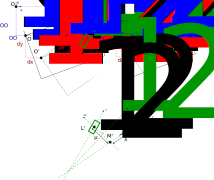
\includegraphics[width=\linewidth]{glissiere.pdf}
	\end{center}

	
	On pose :
	
	\parametrageAngulaire{\dtheta1}{\v1}{\w1}{\vz{}}{\v1'}{\w1'}
	\parametrageAngulaire{\dtheta2}{\v2}{\w2}{\vz{}}{\v2'}{\w2'}
	\parametrageAngulaire{(\dtheta1+\dtheta2)/2}{\v{}}{\w{}}{\vz{}}{\v{}'}{\w{}'}
	
        \begin{align*}
            \v{}&=\frac{\v1+\v2}{\norme{\v1+\v2}}    \\
            \w{}&=\frac{\v1-\v2}{\norme{\v1-\v2}}    \\
            \v1'&=\v1+\dtheta1\w1   \\
            \w1'&=\w1-\dtheta1\v1 \\
            \v2'&=\v2+\dtheta2\w2 \\
            \w2'&=\w2-\dtheta2\v2 \\
            \v{}'&=\v{}+\frac{\dtheta1+\dtheta2}{2}\w{}\\
            \w{}'&=\w{}-\frac{\dtheta1+\dtheta2}{2}\v{}\\
            \vDep{L_1}{1}{0}&=\vDep{O_1}{1}{0}+\vecteur{L_1O_1}\wedge\vPetiteRot10\\
            \vDep{L_2}{2}{0}&=\vDep{O_2}{2}{0}+\vecteur{L_2O_2}\wedge\vPetiteRot20\\
        \end{align*}
	
	
	
	\subsection{Force de $L_2$ sur $L_1$}
	% ------------------------------------------------
	
	Note : Pour $\mu$, voir \href{https://math.stackexchange.com/questions/148199/equation-for-non-orthogonal-projection-of-a-point-onto-two-vectors-representing}{ce site}.
	
	
        \begin{align*}
            \resAM{L_2}{L_1}    =&  k\vecteur{L_1'M_2'}   \\
                        =&  -k\mu'\w{}'\\
                        =&  -k\left(\frac{\vz{}\cdot(\v2'\wedge\vecteur{L_1'L_2'})}{\vz{}\cdot(\v2'\wedge\w{}')}\right)\w{}'\\
                        =&  k\left(
                                \frac
                                    {\vz{}\cdot(\vecteur{L_1'L_2'}\wedge\v2')}
                                    {\vz{}\cdot(\underbrace{\v2'\wedge\w{}'}_{\approx\v2\wedge\w{}})}
                            \right)
                               \left(\w{}-\frac{\dtheta1+\dtheta2}{2}\v{}\right) \\
                        =&  k\left(
                                \frac
                                    {\vz{}\cdot\left(\vecteur{L_1'L_2'}\wedge(\v2+\dtheta2\w2)\right)}
                                    {\vz{}\cdot(\v2\wedge\w{})}%\left((\v2+\dtheta2\w2)\wedge\left(\w{}-\frac{\dtheta1+\dtheta2}{2}\v{}\right)\right)}
                            \right)
                               \left(\w{}-\frac{\dtheta1+\dtheta2}{2}\v{}\right) \\
                        =&  k\left(
                                \frac
                                    {\vz{}\cdot\left(\left(\vecteur{L_1'L_1}+\vecteur{L_1L_2}+\vecteur{L_2L_2'}\right)\wedge(\v2+\dtheta2\w2)\right)}
                                    {\vz{}\cdot(\v2\wedge\w{})}
                            \right)
                               \left(\w{}-\frac{\dtheta1+\dtheta2}{2}\v{}\right)\\
                        =&  k\left(
                                \frac
                                    {\vz{}\cdot\left(\left(-\vDep{L_1}{1}{0}+\vecteur{L_1L_2}+\vDep{L_2}{2}{0}\right)\wedge(\v2+\dtheta2\w2)\right)}
                                    {\vz{}\cdot(\v2\wedge\w{})}
                            \right)
                               \left(\w{}-\frac{\dtheta1+\dtheta2}{2}\v{}\right)
        \end{align*}
        \begin{align*}
                        =&  k\left(
                                \frac
                                    {\vz{}\cdot\left(\overbrace{\left(-\vDep{O_1}{1}{0}-\vecteur{L_1O_1}\wedge\vPetiteRot10+\vecteur{L_1L_2}+\vDep{O_2}{2}{0}+\vecteur{L_2O_2}\wedge\vPetiteRot20\right)\wedge(\v2+\dtheta2\w2)}^{A}\right)}
                                    {\vz{}\cdot(\v2\wedge\w{})}
                            \right)\\
                            &\times
                               \left(\w{}-\frac{\dtheta1+\dtheta2}{2}\v{}\right)
        \end{align*}
        
        Développons $A$, en simplifiant les termes dont le produit sera très petit (exemple : $\dtheta2\times\dx2$) :
        
        \begin{align*}
            A =& \left(-\vDep{O_1}{1}{0}-\vecteur{L_1O_1}\wedge\vPetiteRot10+\vecteur{L_1L_2}+\vDep{O_2}{2}{0}+\vecteur{L_2O_2}\wedge\vPetiteRot20\right)\wedge(\v2+\dtheta2\w2)    \\
            =&  \left(-\vDep{O_1}{1}{0}-\vecteur{L_1O_1}\wedge\vPetiteRot10+\vecteur{L_1L_2}+\vDep{O_2}{2}{0}+\vecteur{L_2O_2}\wedge\vPetiteRot20\right)\wedge\v2\\
            &+\left(-\underbrace{\cancel{\vDep{O_1}{1}{0}}}_{\approx0}-\underbrace{\cancel{\vecteur{L_1O_1}\wedge\vPetiteRot10}}_{\approx0}+\vecteur{L_1L_2}+\underbrace{\cancel{\vDep{O_2}{2}{0}}}_{\approx0}+\underbrace{\cancel{\vecteur{L_2O_2}\wedge\vPetiteRot20}}_{\approx0}\right)\wedge(\dtheta2\w2)\\
            =&
            \left(
                \begin{array}{r}
                    -\dx1-L_1O_1\py\times\dtheta1+L_1L_2\px+\dx2+L_2O_2\py\times\dtheta2
                    \\
                    -\dy1+L_1O_1\px\times\dtheta1+L_1L_2\py+\dy2-L_2O_2\px\times\dtheta2
                 \end{array}
            \right)\wedge\v2
            +\dtheta2\left(L_1L_2\px\times w_2\py-L_1L_2\py\times w_2\px\right)\vz{}\\
            =&\left[\left(-\dx1-L_1O_1\py\times\dtheta1+L_1L_2\px+\dx2+L_2O_2\py\times\dtheta2\right)\times v_2\py\right.
                    \\
                    &-\left(-\dy1+L_1O_1\px\times\dtheta1+L_1L_2\py+\dy2-L_2O_2\px\times\dtheta2\right)\times v_2\px
                    \\
                    &\left.+\dtheta2\left(L_1L_2\px\times w_2\py-L_1L_2\py\times w_2\px\right)\right]\vz{}
        \end{align*}
        
    Donc :
    \begin{align*}
            \resAM{L_2}{L_1}    =&  \frac{k}{\vz{}\cdot\left(\v2\wedge\w{}\right)}
                                    \left[
                                        \left(-\dx1-\dtheta1L_1O_1\py+L_1L_2\px+\dx2+\dtheta2L_2O_2\py\right)\times v_2\py\
                                    \right.
                                        \\
                                        &+\left(\dy1-\dtheta1L_1O_1\px-L_1L_2\py-\dy2+\dtheta2L_2O_2\px\right)\times v_2\px
                                        \\
                                   & \left.
                                        +\dtheta2\left(L_1L_2\px\times w_2\py-L_1L_2\py\times w_2\px\right)
                                    \right]   \\
                                    &\times\left(\begin{array}{c}
                                        w\px-\frac{\dtheta1+\dtheta2}{2}v\px
                                        \\
                                        w\py-\frac{\dtheta1+\dtheta2}{2}v\py
                                    \end{array}\right)\\
                                =&\overbrace{\frac{k}{v_2\px\ w\py-v_2\py\ w\px}}^B\times \\
                                &\left[(-v_2\py) \dx1 + (v_2\px)\dy1+(-v_2\py L_1O_1\py+v_2\px L_1O_1\px)\dtheta1\right.\\
                                &+(v_2\py)\dx2-(v_2\px)\dy2+(v_2\py L_2O_2\py+v_2\px L_2O_2\px+L_1L_2\px w_2\py-L_1L_2\py w_2\px)\dtheta2\\
                                &\left.+\underbrace{L_1L_2\px\ v_2\py-L_1L_2\py\ v_2\px}_{C}\right]\\
                                    &\times\left(\begin{array}{c}
                                        w\px-\frac{\dtheta1+\dtheta2}{2}v\px
                                        \\
                                        w\py-\frac{\dtheta1+\dtheta2}{2}v\py
                                    \end{array}\right)\\
                                =&  B\times\\
                                &\left[\left(
                                    \begin{array}{l}
                                        (-v_2\py w\px) \dx1 + (v_2\px w\px)\dy1+(-v_2\py L_1O_1\py+v_2\px L_1O_1\px)w\px\dtheta1+(v_2\py w\px)\dx2\dots \\
                                        (-v_2\py w\py) \dx1 + (v_2\px w\py)\dy1+(-v_2\py L_1O_1\py+v_2\px L_1O_1\px) w\py\dtheta1+(v_2\py w\py)\dx2\dots
                                    \end{array}
                                \right.\right.\\
                                &\left.
                                    \begin{array}{l}
                                        \dots-(v_2\px w\px)\dy2+(v_2\py L_2O_2\py+v_2\px L_2O_2\px+L_1L_2\px w_2\py-L_1L_2\py w_2\px) w\px\dtheta2+Cw\px\\
                                        \dots-(v_2\px w\py)\dy2+(v_2\py L_2O_2\py+v_2\px L_2O_2\px+L_1L_2\px w_2\py-L_1L_2\py w_2\px) w\py\dtheta2+Cw\py
                                    \end{array}
                                \right)
                                \\
                                &\left.+\left(
                                    \begin{array}{c}
                                        -\frac{Cv\px}{2}\dtheta1
                                        -\frac{Cv\px}{2}\dtheta2
                                        \\
                                        -\frac{Cv\py}{2}\dtheta1
                                        -\frac{Cv\py}{2}\dtheta2
                                    \end{array}
                                \right)\right]
    \end{align*}
    
    
	\subsection{Moment en $O_1'$ de $L_2$ sur $L_1$}
	% ------------------------------------------------
	
	Appelons $\vecteur{C_{L_2\mapsto L_1}}$ le couple du ressort de torsion de liaison.
	
	\begin{align*}
        \momAM{O_1'}{2}{1}\cdot \vz{}  =&
            \vecteur{C_{L_2\mapsto L_1}}\cdot\vz{}+\left(\vecteur{O_1'L_1'}\wedge \resAM{2}{1}\right)\cdot\vz{}  \\
            =&
                \krot (\alpha_2+\dtheta2+\theta_2-\alpha_1-\dtheta1-\theta_1)\\
            &+\left(-\vDep{O_1}{1}{0}+\vecteur{O_1L_1}+\vDep{L_1}{1}{0}\right)\wedge
                \text{(Voir résultante)}\cdot\vz{}    \\
            =&    \krot (\alpha_2+\dtheta2+\theta_2-\alpha_1-\dtheta1-\theta_1)\\
            &+\left(-\cancel{\vDep{O_1}{1}{0}}+\vecteur{O_1L_1}+\cancel{\vDep{O_1}{1}{0}}-\vecteur{O_1L_1}\wedge\vPetiteRot10\right)\wedge
                \text{(Voir résultante)} \cdot \vz{}   \\
            =&    \krot (\alpha_2+\dtheta2+\theta_2-\alpha_1-\dtheta1-\theta_1)\\
            &+\left(
                    \begin{array}{c}
                        O_1L_1\px   -   O_1L_1\py\dtheta1   
                        \\O_1L_1\py +   O_1L_1\px\dtheta1
                    \end{array}
                \right)\wedge
                \text{(Voir résultante)} \cdot \vz{}   \\
            %
            =& \krot (\alpha_2+\dtheta2+\theta_2-\alpha_1-\dtheta1-\theta_1)\\
            +B\times[&\\
            &(-v_2\py w\py\ O_1L_1\px)\dx1+(v_2\px w\py O_1L_1\px)\dy1\\
            &+O_1L_1\px\left[(-v_2\py L_1O_1\py+v_2\px L_1O_1\px)w\py-\frac 12 C v\py\right]\dtheta1\\
            &+(v_2\py w\py O_1L_1\px)\dx2-(v_2\px w\py O_1L_1\px)\dy2\\
            &+O_1L_1\px\left[(v_2\py L_2O_2\py+v_2\px L_2O_2\px+L_1L_2\px w_2\py-L_1L_2\py w_2\px)w\py-\frac12 C v\py\right]\dtheta2\\
            &+(Cw\py O_1L_1\px)\\
            &-(O_1L_1\py Cw\py)\dtheta1\\
            &+(v_2\py w\px O_1L_1\py)\dx1
            -(v_2\px w\px O_1L_1\py)\dy1\\
            &+O_1L_1\py\left[(v_2\py L_1O_1\py-v_2\px L_1O_1\px)w\px+\frac 12Cv\px\right]\dtheta1\\
            &-(v_2\py w\px O_1L_1\py)\dx2+(v_2\px w\px O_1L_1\py)\dy2\\
            &+O_1L_1\py\left[(-v_2\py L_2O_2\py-v_2\px L_2O_2\px-L_1L_2\px w_2\py+L_1L_2\py w_2\px)w\px+\frac12 C v\px\right]\dtheta2\\
            &-(O_1L_1\py C w\px)\\
            &-(O_1L_1\px C w\px) \dtheta1\\
            ]&
	\end{align*}


    
	\subsection{Matrices de $L_1$}
	% ------------------------------------------------
	On met les actions mécaniques précédentes sous la forme :
        \begin{align}
                                =&\bar {\bar A}\cdot \vecteur X-\vecteur F
        \end{align}
avec
    \begin{align*}
        \vecteur X  &=  \left(
                            \begin{array}{c}
                                \dx1\\\dy1\\\dtheta1\\\dx2\\\dy2\\\dtheta2
                            \end{array}
                        \right)
    \end{align*}

    
    \begin{align*}
        \bar{\bar A} =&
        \left[
            \begin{array}{cccc}
                (-B\ v_2\py w\px)     &      (B\ v_2\px w\px)      & \dots  \\
                (-B\ v_2\py w\py)     &     (B\ v_2\px w\py)        & \dots \\
                Bv_2\py(w\px O_1L_1\py-w\py O_1L_1\px)       &       Bv_2\px(w\py O_1L_1\px-w\px O_1L_1\py)   & \dots \\
            \end{array}
        \right.\\[0.5cm]
        &
        \left|
            \begin{array}{ccc}
                \dots & B\left((-v_2\py L_1O_1\py+v_2\px L_1O_1\px)w\px-\frac{Cv\px}{2}\right)    &\dots  \\
                %
                \dots   &   B\left((-v_2\py L_1O_1\py+v_2\px L_1O_1\px) w\py-\frac{Cv\py}{2}\right)    &\dots\\
                %
                   \dots & \scalemath{0.65}{
                    \tiny -\krot+B\left(O_1L_1\px\left[(-v_2\py L_1O_1\py+v_2\px L_1O_1\px)w\py-\frac 12 C v\py\right] -(O_1L_1\py Cw\py)  +O_1L_1\py\left[(v_2\py L_1O_1\py-v_2\px L_1O_1\px)w\px+\frac 12Cv\px\right] -(O_1L_1\px C w\px) \right)
                    }&\dots
            \end{array}
        \right.\\[0.5cm]
        &\left|
            \begin{array}{cccc}
                \dots   &   (Bv_2\py w\px)   &   -(B\ v_2\px w\px) &     \dots\\
                \dots   &   (B\ v_2\py w\py)   &  -(B\ v_2\px w\py)     &   \dots\\
                \dots   &   Bv_2\py (w\py O_1L_1\px- w\px O_1L_1\py)   &   Bv_2\px( w\px O_1L_1\py- w\py O_1L_1\px)   &   \dots
            \end{array}
        \right.\\[0.5cm]
        &\left.
            \begin{array}{cc}
                \dots   &     B\left((v_2\py L_2O_2\py+v_2\px L_2O_2\px+L_1L_2\px w_2\py-L_1L_2\py w_2\px) w\px-\frac{Cv\px}{2}\right)\\
                \dots   &   B\left((v_2\py L_2O_2\py+v_2\px L_2O_2\px+L_1L_2\px w_2\py-L_1L_2\py w_2\px) w\py-\frac{Cv\py}{2}\right)\\
                \dots     &   \scalemath{0.6}{
                    \krot +B\left(O_1L_1\px\left[(v_2\py L_2O_2\py+v_2\px L_2O_2\px+L_1L_2\px w_2\py-L_1L_2\py w_2\px)w\py-\frac12 C v\py\right] +O_1L_1\py\left[(-v_2\py L_2O_2\py-v_2\px L_2O_2\px-L_1L_2\px w_2\py+L_1L_2\py w_2\px)w\px+\frac12 C v\px\right]   \right)
                }
            \end{array}
        \right]
    \end{align*}
    
    \begin{align*}
        \vecteur F &= \left(\begin{array}{c}
                                -B\ C\ w\px
                                \\
                                -B\ C\ w\py
                                \\
                                \krot (\alpha_1+\theta_1-\alpha_2-\theta_2)+B\ C(w\px O_1L_1.y-w\py O_1L_1\px)
                            \end{array}\right)
    \end{align*}



    
    
    
    
    %%%%%%%%%%%%%%%%%%%%%%%%%%%%%%%%%%%%%%%%%%%%%%%%%%%%%%%%%%%%
    %%%%%%%%%%%%%%%%%%%%%%%%%%%%%%%%%%%%%%%%%%%%%%%%%%%%%%%%%%%%
    %%%%%%%%%%%%%%%%%%%%%%%%%%%%%%%%%%%%%%%%%%%%%%%%%%%%%%%%%%%%
    %%%%%%%%%%%%%%%%%%%%%%%%%%%%%%%%%%%%%%%%%%%%%%%%%%%%%%%%%%%%
    %%%%%%%%%%%%%%%%%%%%%%%%%%%%%%%%%%%%%%%%%%%%%%%%%%%%%%%%%%%%
    %%%%%%%%%%%%%%%%%%%%%%%%%%%%%%%%%%%%%%%%%%%%%%%%%%%%%%%%%%%%
    
    \subsection{Force de $L_1$ sur $L_2$}
	% ------------------------------------------------

        La force est strictement l'opposée :
        
        \begin{align*}
            \resAM{L_1}{L_2}=&-\resAM{L_2}{L_1}\\
                    =& -B\times\\
                                &\left[\left(
                                    \begin{array}{l}
                                        (-v_2\py w\px) \dx1 + (v_2\px w\px)\dy1+(-v_2\py L_1O_1\py+v_2\px L_1O_1\px)w\px\dtheta1+(v_2\py w\px)\dx2\dots \\
                                        (-v_2\py w\py) \dx1 + (v_2\px w\py)\dy1+(-v_2\py L_1O_1\py+v_2\px L_1O_1\px) w\py\dtheta1+(v_2\py w\py)\dx2\dots
                                    \end{array}
                                \right.\right.\\
                                &\left.
                                    \begin{array}{l}
                                        \dots-(v_2\px w\px)\dy2+(v_2\py L_2O_2\py+v_2\px L_2O_2\px+L_1L_2\px w_2\py-L_1L_2\py w_2\px) w\px\dtheta2+Cw\px\\
                                        \dots-(v_2\px w\py)\dy2+(v_2\py L_2O_2\py+v_2\px L_2O_2\px+L_1L_2\px w_2\py-L_1L_2\py w_2\px) w\py\dtheta2+Cw\py
                                    \end{array}
                                \right)
                                \\
                                &\left.+\left(
                                    \begin{array}{c}
                                        -\frac{Cv\px}{2}\dtheta1
                                        -\frac{Cv\px}{2}\dtheta2
                                        \\
                                        -\frac{Cv\py}{2}\dtheta1
                                        -\frac{Cv\py}{2}\dtheta2
                                    \end{array}
                                \right)\right]
        \end{align*}


    \subsection{Moment en $O_2'$ de $L_1$ sur $L_2$}
	% ------------------------------------------------
	
        Appelons $\vecteur{C_{L_1\mapsto L_2}}=-\vecteur{C_{L_2\mapsto L_1}}$ le couple du ressort de torsion de liaison.
        
        \begin{align*}
            \momAM{O_2'}{1}{2}\cdot \vz{}   =& \vecteur{C_{L_1\mapsto L_2}}\cdot \vz{}  + \left(\underbrace{\vecteur{O_2'M_2'}}_{\text{(ou \vecteur{O_2'L_1'})}}\wedge\resAM{1}{2}\right)\cdot\vz{}\\
                        =& \krot (\alpha_1+\dtheta1+\theta_1-\alpha_2-\dtheta2-\theta_2)\\
                        &+\left(\left(\vecteur{O_2'O_2}+\vecteur{O_2L_1}+\vecteur{L_1L_1'}\right)\wedge(\text{Voir résultante})\right)\cdot\vz{}\\
                        =& \krot (\alpha_1+\dtheta1+\theta_1-\alpha_2-\dtheta2-\theta_2)\\
                        &+\left(\left(-\vDep{O_2}{2}{0}+\vecteur{O_2L_1}+\vDep{L_1}{1}{0}\right)\wedge(\text{Voir résultante})\right)\cdot\vz{}\\
                        =& \krot (\alpha_1+\dtheta1+\theta_1-\alpha_2-\dtheta2-\theta_2)\\
                        &+\left(\left(-\vDep{O_2}{2}{0}+\vecteur{O_2L_1}+\vDep{O_1}{1}{0}+\vecteur{L_1O_1}\wedge\vPetiteRot10\right)\wedge(\text{Voir résultante})\right)\cdot\vz{}\\
                        =& \krot(\alpha_1+\dtheta1+\theta_1-\alpha_2-\dtheta2-\theta_2)\\
                        &+\left(\left(
                            \begin{array}{c}
                                -\dx2 + O_2L_1\px + \dx1 + L_1O_1\py\dtheta1
                                \\
                                -\dy2 + O_2L_1\py + \dy1 - L_1O_1\px\dtheta1
                            \end{array}
                        \right)\wedge(\text{Voir résultante})\right)\cdot\vz{}\\
                        =&  \krot(\alpha_1+\dtheta1+\theta_1-\alpha_2-\dtheta2-\theta_2)\\
                        -B [&\\
                        &
                                (Cw\py)\dx1
                                -(Cw\py)\dx2
                                +(L_1O_1\py Cw\py)\dtheta1
                            \\
                            &%
                                -(O_2L_1\px v_2\py w\py)\dx1
                                +(O_2L_1\px v_2\px w\py)\dy1
                                \\&
                                +\left(O_2L_1\px \left((-v_2\py L_1O_1\py+v_2\px L_1O_1\px)w\py-\frac 12 Cv\py\right)\right)\dtheta1
                                \\&
                                +(O_2L_1\px v_2\py w\py)\dx2
                                -(O_2L_1\px v_2\px w\py)\dy2
                                \\
                                &+\left(O_2L_1\px \left((v_2\py L_2O_2\py+v_2\px L_2O_2\px+L_1L_2\px w_2\py-L_1L_2\py w_2\px)w\py-\frac12 Cv\py\right)\right)\dtheta2\\
                                &+(O_2L_1\px C w\py)
                                \\%
                                %
                                &-(Cw\px)\dy1
                                +(Cw\px)\dy2
                                +(L_1O_1\px Cw\px)\dtheta1
                                \\
                                &+(O_2L_1\py v_2\py w\px)\dx1
                                -(O_2L_1\py v_2\px w\px)\dy1\\
                                &-\left(O_2L_1\py\left((-v_2\py L_1O_1\py+v_2\px L_1O_1\px)w\px-\frac 12 C v\px\right)\right)\dtheta1\\
                                &-(O_2L_1\py v_2\py w\px)\dx2
                                +(O_2L_1\py v_2\px w\px)\dy2\\
                                &-\left(O_2L_1\py\left((v_2\py L_2O_2\py+v_2\px L_2O_2\px+L_1L_2\px w_2\py-L_1L_2\py w_2\px)w\px-\frac 12 C v\px\right)\right)\dtheta2
                                \\
                                &-(O_2L_1\py Cw\px)
                                \\  
                        ]&
        \end{align*}

	
	
	\subsection{Matrices de $L_2$}
	% ------------------------------------------------
	On met les actions mécaniques précédentes sous la forme :
        \begin{align}
                                =&\bar {\bar A}\cdot \vecteur X-\vecteur F
        \end{align}
avec (attention à l'ordre !)
    \begin{align*}
        \vecteur X  &=  \left(
                            \begin{array}{c}
                                \dx1\\\dy1\\\dtheta1\\\dx2\\\dy2\\\dtheta2
                            \end{array}
                        \right)
    \end{align*}
    
     \begin{align*}
        \bar{\bar A} =&
        \left[
            \begin{array}{cccc}
               (B\ v_2\py w\px)     &      (-B\ v_2\px w\px)      & \dots  \\
                (B\ v_2\py w\py)     &     (-B\ v_2\px w\py)        & \dots \\
                -B(Cw\py+O_2L_1\px v_2\py w\py)     &       -B(O_2L_1\px v_2\px w\py-C w\px-O_2L_1\py v_2\px w\px)   & \dots \\
            \end{array}
        \right.\\[0.5cm]
        &
        \left|
            \begin{array}{ccc}
                \dots & -B\left((-v_2\py L_1O_1\py+v_2\px L_1O_1\px)w\px-\frac{Cv\px}{2}\right)    &\dots  \\
                %
                \dots   &   -B\left((-v_2\py L_1O_1\py+v_2\px L_1O_1\px) w\py-\frac{Cv\py}{2}\right)    &\dots\\
                %
                   \dots & \scalemath{0.65}{\left(\krot-B\left[
                            L_1O_1\py Cw\py
                            + O_2L_1\px \left((-v_2\py L_1O_1\py+v_2\px L_1O_1\px)w\py-\frac 12 Cv\py\right)
                            +L_1O_1\px Cw\px
                            -O_2L_1\py\left((-v_2\py L_1O_1\py+v_2\px L_1O_1\px)w\px-\frac 12 C v\px\right)
                        \right]\right)}    &\dots
            \end{array}
        \right.\\[0.5cm]
        &\left|
            \begin{array}{cccc}
                \dots   &   (-Bv_2\py w\px)   &   (B\ v_2\px w\px) &     \dots\\
                \dots   &   (-B\ v_2\py w\py)   &  (B\ v_2\px w\py)     &   \dots\\
                \dots   &   -B(-C w\py+O_2L_1\px v_2\py w\py-O_2L_1\py v_2\py w\px)   &   -B(-O_2L_1\px v_2\px w\py+O_2L_1\py v_2\px w\px)  &   \dots
            \end{array}
        \right.\\[0.5cm]
        &\left.
            \begin{array}{cc}
                \dots   &     -B\left((v_2\py L_2O_2\py+v_2\px L_2O_2\px+L_1L_2\px w_2\py-L_1L_2\py w_2\px) w\px-\frac{Cv\px}{2}\right)\\
                \dots   &   -B\left((v_2\py L_2O_2\py+v_2\px L_2O_2\px+L_1L_2\px w_2\py-L_1L_2\py w_2\px) w\py-\frac{Cv\py}{2}\right)\\
%                 \dots     &   \scalemath{0.65}{\left(
%                                     -\krot -B\left[
%                                         O_2L_1\px \left((v_2\py L_2O_2\py+v_2\px L_2O_2\px+L_1L_2\px w_2\py-L_1L_2\py w_2\px)w\py-\frac12 Cv\py\right)
%                                     -O_2L_1\py\left((v_2\py L_2O_2\py+v_2\px L_2O_2\px+L_1L_2\px w_2\py-L_1L_2\py w_2\px)w\px-\frac 12 C v\px\right)\right)
%                                     \right]
%                             \right)}
%                 \\
                 \dots &       \scalemath{0.65}{-\krot-B\left[
                                            (v_2\py L_2O_2\py+v_2\px L_2O_2\px+L_1L_2\px w_2\py-L_1L_2\py w_2\px) (O_2L_1\px w\py-O_2L_1\py w\px)
                                            +\frac 12 C(O_2L_1\px v\py-O_2L_1\py v\px)
%                  
%                  
%                                         O_2L_1\px \left((v_2\py L_2O_2\py+v_2\px L_2O_2\px+L_1L_2\px w_2\py-L_1L_2\py w_2\px)w\py-\frac12 Cv\py\right)
%                                     -O_2L_1\py\left((v_2\py L_2O_2\py+v_2\px L_2O_2\px+L_1L_2\px w_2\py-L_1L_2\py w_2\px)w\px-\frac 12 C v\px\right)\right)
                             \right]}
            \end{array}
        \right]
    \end{align*}
    
    \begin{align*}
        \vecteur F &= \left(\begin{array}{c}
                                B\ C\ w\px
                                \\
                                B\ C\ w\py
                                \\
                               \krot(-\alpha_1+-\theta_1+\alpha_2+\theta_2)+B\ C(O_2L_1\px w\px-O_2L_1\py w\py)
                            \end{array}
                            \right)
    \end{align*}

\end{document}
